% DCGAN 论文简单解读
%   https://www.cnblogs.com/lyrichu/p/9054704.html

% Unsupervised Representation Learning with Deep Convolutional Generative Adversarial Networks
%   https://arxiv.org/abs/1511.06434


\documentclass[a4paper, 12pt]{article}
\usepackage[UTF8]{ctex}
% \usepackage[T1]{fontenc}
% \usepackage{inconsolata}

\usepackage[hidelinks]{hyperref}

\usepackage{amsmath}
\usepackage{enumitem}
\setlist{
    nolistsep, % 去掉 item 和正文之间的间隔
    % labelindent=\parindent,
    leftmargin=*, % 保证小节标签缩进和上面对齐
    % labelsep=1em, % 标签后的空白
    align=left, % 标签对齐段落左边缘
}
\usepackage{tabularx}

\usepackage{graphicx}
\usepackage{subfig}
% \usepackage{subcaption}

\usepackage{geometry}
\geometry{
    a4paper,
    left=2cm,
    right=2cm,
    top=2cm,
    bottom=2cm,
}

\newcommand{\fs}[1]{\fontsize{#1 pt}{0pt}\selectfont}

\usepackage{mathtools}
\DeclarePairedDelimiter{\ceil}{\lceil}{\rceil}
\DeclarePairedDelimiter\floor{\lfloor}{\rfloor}

\usepackage{setspace}
% \setlength\parindent{0pt}
\setlength{\parindent}{2em} % 中文

% \newfontfamily\csl{Consolas}

\usepackage{array}
\newcolumntype{T}{>{\ttfamily}l}
\newcolumntype{Y}{>{\footnotesize\ttfamily}l}
\newcolumntype{y}{>{\footnotesize\ttfamily}c}

\usepackage{longtable}

\newcommand*{\thead}[1]{\multicolumn{1}{c}{\bfseries #1}}
\newcommand*{\yhead}[1]{\multicolumn{1}{c}{\footnotesize\bfseries #1}}

\newcommand{\ssa}{\phantom{x}}
\newcommand{\ssb}{\phantom{xx}}
\newcommand{\ssc}{\phantom{xxx}}
\newcommand{\ssd}{\phantom{xxxx}}
\newcommand{\sse}{\phantom{xxxxx}}

\usepackage{xcolor}
\usepackage{listings}
\definecolor{mygreen}{RGB}{28,172,0} % color values Red, Green, Blue
\definecolor{mylilas}{RGB}{170,55,241}

\newcommand{\ttf}{\ttfamily}

\lstdefinestyle{plainText}{language={},
    basicstyle=\footnotesize \ttfamily,        % set font type and size
    % basicstyle=\ttfamily,        % set font type and size
    breaklines=true,
    keywordstyle=\color{blue},
    % morekeywords={matlab2tikz},
    % morekeywords=[2]{1}, 
    % keywordstyle=[2]{\color{black}},
    identifierstyle=\color{black},
    stringstyle=\color{mylilas},
    % stringstyle=\color{purple},
    frame=single,
    framexleftmargin=0em,
    aboveskip=-\baselineskip,
    commentstyle=\color{mygreen},
    showstringspaces=false,% without this there will be a symbol in the places where there is a space
    % numbers=left,
    numbers=none,
    numberstyle={\tiny \color{black}}, % size of the numbers
    numbersep=9pt, % this defines how far the numbers are from the text
    tabsize=4,                     % sets default tabsize to 4 spaces
    emph=[1]{},
    emphstyle=[1]\color{blue}, %some words to emphasise
    %emph=[2]{word1,word2}, 
    % emphstyle=[2]{style}, 
    escapeinside=``,               % Characters escape: To Use Chinese in codes   
}

\lstdefinestyle{myC}{language={C},
    % basicstyle=\footnotesize \ttfamily,        % set font type and size
    basicstyle=\ttfamily,        % set font type and size
    breaklines=true,
    keywordstyle=\color{blue},
    % morekeywords={matlab2tikz},
    % morekeywords=[2]{1}, 
    % keywordstyle=[2]{\color{black}},
    identifierstyle=\color{black},
    stringstyle=\color{mylilas},
    % stringstyle=\color{purple},
    frame=single,
    framexleftmargin=0em,
    aboveskip=-\baselineskip,
    commentstyle=\color{mygreen},
    showstringspaces=false,% without this there will be a symbol in the places where there is a space
    % numbers=left,
    numbers=none,
    numberstyle={\tiny \color{black}}, % size of the numbers
    numbersep=9pt, % this defines how far the numbers are from the text
    tabsize=4,                     % sets default tabsize to 4 spaces
    emph=[1]{function, return, f, let, add, mult, dot, rk, uw2uwdd, uw2xy1, uw2xy2},
    emphstyle=[1]\color{blue}, %some words to emphasise
    % emph=[2]{word1,word2}, 
    % emphstyle=[2]{style}, 
    escapeinside=``,               % Characters escape: To Use Chinese in codes   
}


\lstdefinestyle{myPython}{language=Python,
    % basicstyle=\footnotesize \ttconsolas,        % set font type and size
    basicstyle=\footnotesize \ttfamily,        % set font type and size
    breaklines=true,
    keywordstyle=\color{blue},
    % morekeywords={matlab2tikz},
    % morekeywords=[2]{1}, 
    % keywordstyle=[2]{\color{black}},
    identifierstyle=\color{black},
    stringstyle=\color{mylilas},
    % stringstyle=\color{purple},
    frame=single,
    framexleftmargin=0em,
    aboveskip=-\baselineskip,
    commentstyle=\color{mygreen},
    showstringspaces=false,% without this there will be a symbol in the places where there is a space
    numbers=left,
    numberstyle={\tiny \color{black}}, % size of the numbers
    numbersep=9pt, % this defines how far the numbers are from the text
    tabsize=4,                     % sets default tabsize to 4 spaces
    emph=[1]{nonLinearFunction, bitReorganization, modAdd_2e31m1, binaryAdd, binaryXor, sboxOfZuc, linearTransform},
    emphstyle=[1]\color{red}, %some words to emphasise
    %emph=[2]{word1,word2}, 
    % emphstyle=[2]{style}, 
    escapeinside=``,               % Characters escape: To Use Chinese in codes   
}



\begin{document}

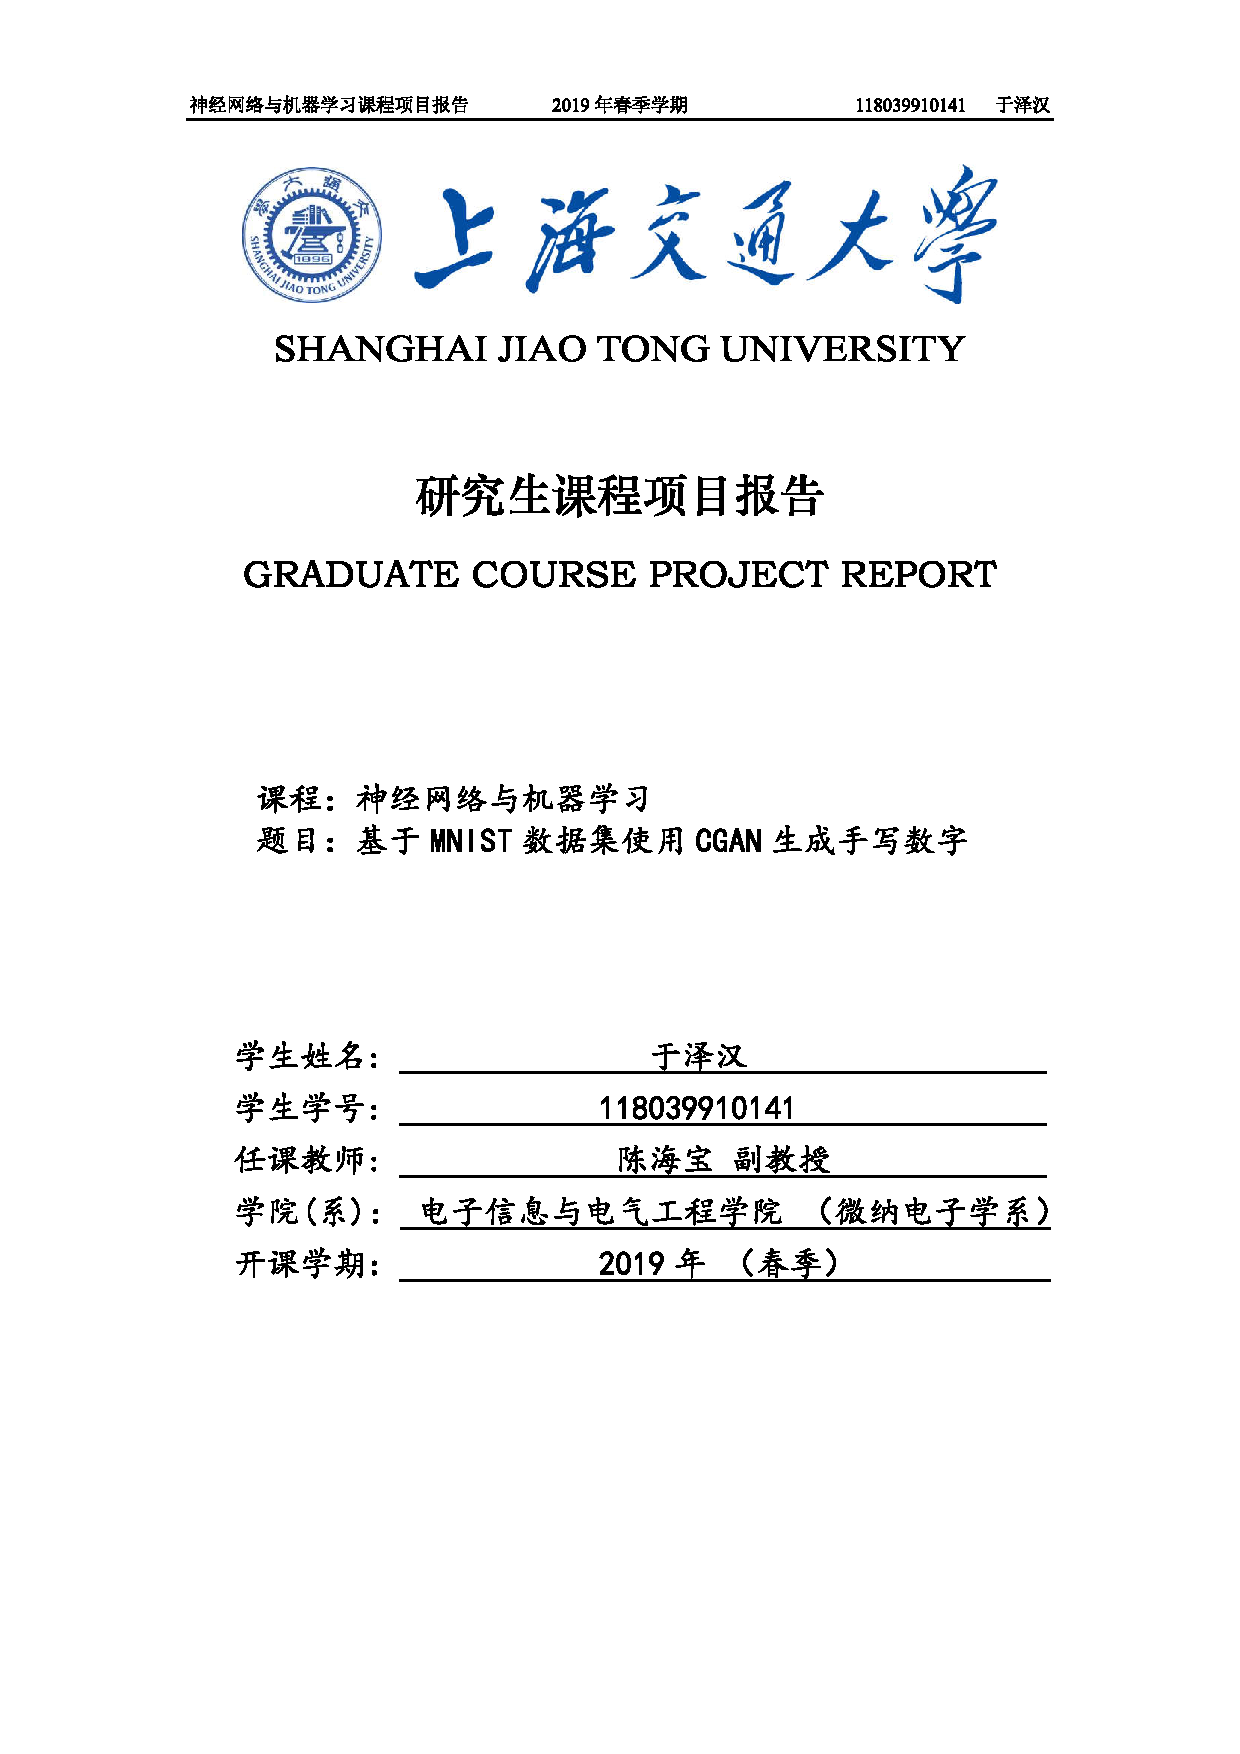
\includepdf[]{./images/cover.pdf}


% 题目、摘要、问题描述、模型建立与求解过程、代码实现、结果与分析、参考文献
% 期末报告基本要求:(1)模型建立和理论求解过程。例如,数据的处理方式?求解方法的选择?参数的控制和调节? (2)代码实现过程:原始代码+代码注释+结果展示,需说明运行平台。


\section{摘要}
在近年的计算机视觉应用中,卷积神经网络(CNN)的监督学习颇受青睐,而无监督学习相关的研究较少。

就在这时,DCGAN(深度卷积生成对抗网络)应运而生,诸多研究和实验证明,它们是无监督学习的有力候选者,弥补了计算机视觉领域中监督学习和无监督学习之间的鸿沟。

在研究者提出 DCGAN 之后,人们用它做了进一步的研究和更多的实验。这一网络结构在训练各种图像数据集时展现出了优异的能力,从物体的局部到整个场景,生成器和判别器都学习到了丰富的层次表达。

\section{模型建立与代码实现}


\begin{lstlisting}[style=myPython,caption={导入必要的库}]
import tensorflow as tf
tf.enable_eager_execution()

import glob
import imageio
import matplotlib.pyplot as plt
import numpy as np
import os
import PIL
import time

from IPython import display
\end{lstlisting}

\subsection{导入数据集}
本次实验采用的是 MNIST 数据集。

\begin{lstlisting}[style=myPython,caption={导入数据集}]
(train_images, train_labels), (_, _) = tf.keras.datasets.mnist.load_data()
\end{lstlisting}

查看数据集的信息:

\begin{lstlisting}[style=myPython,caption={查看数据集信息}]
train_images.shape,train_labels.shape
train_labels[0:20]
\end{lstlisting}

输出:

\begin{lstlisting}[style=myPlain]
((60000, 28, 28), (60000,))
array([5, 0, 4, 1, 9, 2, 1, 3, 1, 4, 3, 5, 3, 6, 1, 7, 2, 8, 6, 9], dtype=uint8)
\end{lstlisting}

输出信息表明,该数据集中共有 60000 张图像,每张图像的大小为 $28 \times 28$,单位为像素。这些图像都对应一个标签,标签的数据类型是 8 位无符号整数,也就是是手写数字图像对应实际数字。


接着查看手写图像的内容:

\begin{lstlisting}[style=myPython,caption={查看手写图像}]
row,col = 10,20
fig_dataset = plt.figure(frameon=False)

for i in range(row):
    j,k = 0,0
    while (k<col):
        if train_labels[j]==i:
            fig_dataset.add_subplot(row, col, col*i+k+1)
            plt.imshow(train_images[j],cmap="gray")
            plt.axis('off')
            k += 1
        j += 1

plt.savefig("./report/images/dateset_preview.png", bbox_inches = 'tight', pad_inches=0)
\end{lstlisting}

得到的图像如下:

\begin{figure}[htbp]
\centering
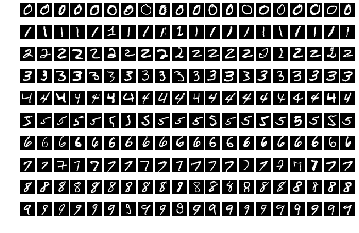
\includegraphics[width=0.8\textwidth]{images/dateset_preview.png}
\caption{手写数字 0 - 9 的图像}
\end{figure}

\begin{lstlisting}[style=myPython,caption={预处理图像数据}]
# `\cmt{将图像像素矩阵尺寸转成 28 x 28}`
train_images = train_images.reshape(train_images.shape[0], 28, 28, 1).astype('float32')
# `\cmt{重映射像素值范围到 [-1, 1]}`
train_images = (train_images - 127.5) / 127.5 
# `\cmt{设置缓存大小}`
BUFFER_SIZE = len(train_labels)
# `\cmt{设置批处理大小}`
BATCH_SIZE = 256
# `\cmt{打乱数据集并设置批处理数目}`
train_dataset = tf.data.Dataset.from_tensor_slices(train_images).shuffle(BUFFER_SIZE).batch(BATCH_SIZE)
\end{lstlisting}

\subsection{创建模型}

\subsubsection{判别器模型}
\begin{lstlisting}[style=myPython,caption={创建判别器模型}]
def make_discriminator_model():
    # `\cmt{采用序贯模型,也就是将多个网络层直接线性堆叠}`
    model = tf.keras.Sequential()

    `\cmt{\color{brown}\# 添加一个卷积层}`
    model.add(tf.keras.layers.Conv2D(64, (5, 5), strides=(2, 2), padding='same'))
    # `\cmt{使用带泄露的线性整流函数}`
    model.add(tf.keras.layers.LeakyReLU())

    `\cmt{\color{brown}\# 添加一个 Dropout 层,随机扔掉部分神经元,避免过拟合}`
    model.add(tf.keras.layers.Dropout(0.3))
      
    `\cmt{\color{brown}\# 添加一个卷积层}`
    model.add(tf.keras.layers.Conv2D(128, (5, 5), strides=(2, 2), padding='same'))
    # `\cmt{使用带泄露的线性整流函数}`
    model.add(tf.keras.layers.LeakyReLU())

    `\cmt{\color{brown}\# 添加一个 Dropout 层}`
    model.add(tf.keras.layers.Dropout(0.3))
    
    `\cmt{\color{brown}\# 添加一个 Flatten 层,连接卷积层和全连接层}`
    model.add(tf.keras.layers.Flatten())

    `\cmt{\color{brown}\# 添加一个全连接层}`
    model.add(tf.keras.layers.Dense(1))
     
    return model

discriminator = make_discriminator_model()
\end{lstlisting}


\subsubsection{生成器模型}
\begin{lstlisting}[style=myPython,caption={创建生成器模型}]
def make_generator_model():
    # `\cmt{采用序贯模型}`
    model = tf.keras.Sequential()

    `\cmt{\color{brown}\# 添加一个全连接层}`
    model.add(tf.keras.layers.Dense(7*7*256, use_bias=False, input_shape=(100,)))
    # `\cmt{对该层进行批标准化,使学习收敛更快更稳}`
    model.add(tf.keras.layers.BatchNormalization())
    # `\cmt{使用带泄露的线性整流函数}`
    model.add(tf.keras.layers.LeakyReLU())

    # `\cmt{调整该层输出的尺寸}`
    model.add(tf.keras.layers.Reshape((7, 7, 256)))
    # `\cmt{检查该层输出的尺寸,这里的 None 表示使用批处理大小}`
    assert model.output_shape == (None, 7, 7, 256) 
    
    `\cmt{\color{brown}\# 添加一个反卷积层}`
    model.add(tf.keras.layers.Conv2DTranspose(128, (5, 5), strides=(1, 1), padding='same', use_bias=False))

    # `\cmt{检查该层输出的尺寸}`
    assert model.output_shape == (None, 7, 7, 128)
    # `\cmt{对该层进行批标准化}`
    model.add(tf.keras.layers.BatchNormalization())
    # `\cmt{使用带泄露的线性整流函数}`
    model.add(tf.keras.layers.LeakyReLU())

    `\cmt{\color{brown}\# 添加一个反卷积层}`
    model.add(tf.keras.layers.Conv2DTranspose(64, (5, 5), strides=(2, 2), padding='same', use_bias=False))
    # `\cmt{检查该层输出的尺寸}`
    assert model.output_shape == (None, 14, 14, 64)
    # `\cmt{对该层进行批标准化}`
    model.add(tf.keras.layers.BatchNormalization())
    # `\cmt{使用带泄露的线性整流函数}`
    model.add(tf.keras.layers.LeakyReLU())

    `\cmt{\color{brown}\# 添加一个反卷积层}`
    model.add(tf.keras.layers.Conv2DTranspose(1, (5, 5), strides=(2, 2), padding='same', use_bias=False, activation='tanh'))
    # `\cmt{检查该层输出的尺寸}`
    assert model.output_shape == (None, 28, 28, 1)

    return model

generator = make_generator_model()
\end{lstlisting}


\subsubsection{损失函数和优化器}

\begin{lstlisting}[style=myPython,caption={判别器损失函数}]
def discriminator_loss(real_output, generated_output):
    # [1,1,...,1] with real output since it is true and we want our generated examples to look like it
    real_loss = tf.losses.sigmoid_cross_entropy(multi_class_labels=tf.ones_like(real_output), logits=real_output)

    # [0,0,...,0] with generated images since they are fake
    generated_loss = tf.losses.sigmoid_cross_entropy(multi_class_labels=tf.zeros_like(generated_output), logits=generated_output)

    total_loss = real_loss + generated_loss

    return total_loss
\end{lstlisting}

\begin{lstlisting}[style=myPython,caption={生成器损失函数}]
def generator_loss(generated_output):
    return tf.losses.sigmoid_cross_entropy(tf.ones_like(generated_output), generated_output)
\end{lstlisting}


\begin{lstlisting}[style=myPython,caption={生成器损失函数}]
learn_rate = 1e-4
generator_optimizer = tf.train.AdamOptimizer(learn_rate)
discriminator_optimizer = tf.train.AdamOptimizer(learn_rate)
\end{lstlisting}

\subsection{训练网络}

\subsubsection{配置网络}

\begin{lstlisting}[style=myPython,caption={配置网络参数}]
EPOCHS = 200
noise_dim = 100
num_examples_to_generate = 16

# We'll re-use this random vector used to seed the generator so
# it will be easier to see the improvement over time.
random_vector_for_generation = tf.random_normal([num_examples_to_generate, noise_dim])
\end{lstlisting}

\begin{lstlisting}[style=myPython,caption={设置训练步骤}]
def train_step(images):
    noise = tf.random_normal([BATCH_SIZE, noise_dim])
      
    with tf.GradientTape() as gen_tape, tf.GradientTape() as disc_tape:
        generated_images = generator(noise, training=True)

        real_output = discriminator(images, training=True)
        generated_output = discriminator(generated_images, training=True)
        
        gen_loss = generator_loss(generated_output)
        disc_loss = discriminator_loss(real_output, generated_output)
        
    gradients_of_generator = gen_tape.gradient(gen_loss, generator.variables)
    gradients_of_discriminator = disc_tape.gradient(disc_loss, discriminator.variables)
      
    generator_optimizer.apply_gradients(zip(gradients_of_generator, generator.variables))
    discriminator_optimizer.apply_gradients(zip(gradients_of_discriminator, discriminator.variables))
train_step = tf.contrib.eager.defun(train_step)
\end{lstlisting}

\begin{lstlisting}[style=myPython,caption={完整训练过程}]
def train(dataset, epochs):  
    for epoch in range(epochs):
        start = time.time()
    
        for images in dataset:
            train_step(images)

        display.clear_output(wait=True)
        generate_and_save_images(generator, epoch + 1, random_vector_for_generation)
    
        print ('Time taken for epoch {} is {} sec'.format(epoch + 1, time.time()-start))
        # generating after the final epoch
    display.clear_output(wait=True)
    generate_and_save_images(generator, epochs, random_vector_for_generation)

%%time
train(train_dataset, EPOCHS)
\end{lstlisting}

\subsection{生成图像}
\begin{lstlisting}[style=myPython,caption={生成图像}]
epoch_images_path = 'epoch_images/'
def generate_and_save_images(model, epoch, test_input):
    # make sure the training parameter is set to False because we
    # don't want to train the batchnorm layer when doing inference.
    predictions = model(test_input, training=False)

    fig = plt.figure(figsize=(4,4))
  
    for i in range(predictions.shape[0]):
        plt.subplot(4, 4, i+1)
        plt.imshow(predictions[i, :, :, 0] * 127.5 + 127.5, cmap='gray')
        plt.axis('off')


    if not os.path.exists(epoch_images_path):
        os.mkdir(epoch_images_path)
    
    plt.savefig(epoch_images_path+'epoch_{:04d}.png'.format(epoch))
    plt.show()

# Display a single image using the epoch number
def display_image(epoch_no):
  return PIL.Image.open(epoch_images_path+'epoch_{:04d}.png'.format(epoch_no))

display_image(EPOCHS)
\end{lstlisting}


\section{结果与分析}
\section{参考文献}


\end{document}

